\section{WebGL}

\subsection{OpenGL Merkmale}

\begin{itemize} \setlength\itemsep{0em}
    \item Low Level Graphics API
    \item Verschiedene Platformen
    \item 1.0/2.0 Fixe Funktionspipeline
    \item Vorlage für WebGL
\end{itemize}

\subsection{Grafikpipeline}

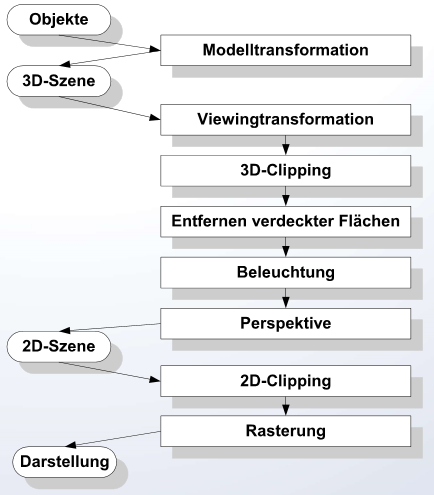
\includegraphics[width=0.4\textwidth]{assets/grafikpipline.png}

\subsection{Programmierbare Shaders}

\textit{
    Shaders werden für die Berechnung der zu zeichnenden
    Objekte verwendet. Das Programm wird direkt auf der Grafikkarte
    ausgeführt.
}

\subsection{Vertex Processing}

\textit{
    Berechnen der Positionen der Vertexe (Punkte) und
    Werte für den folgenden Fragmentshader.
}

\subsection{Fragment Processing}

\textit{
    Berechnet die Farbe der einzelnen Pixel.
}

\subsection{Datenfluss}

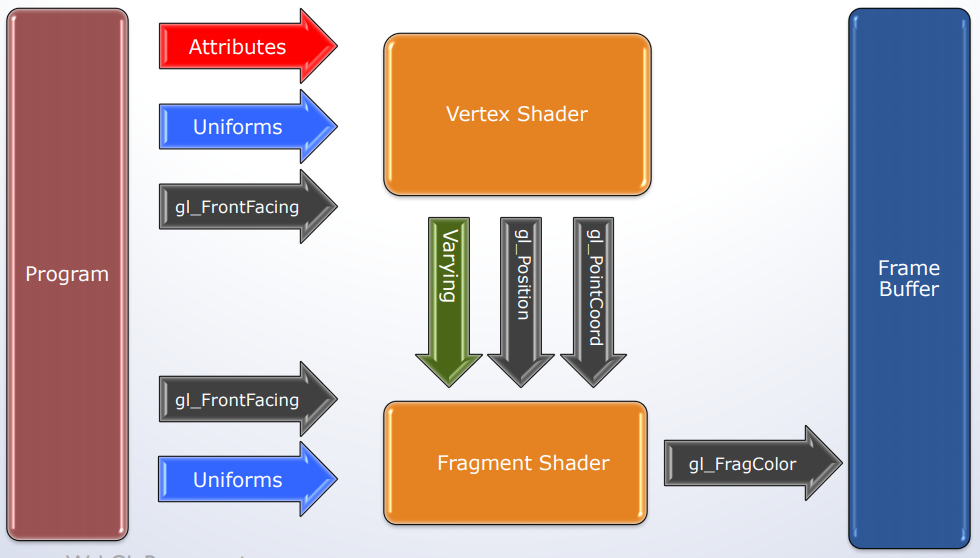
\includegraphics[width=0.5\textwidth]{assets/dataprocessing.png}

\subsection{Attribut Variablen und Buffer definieren}

\textbf{Erzeugen}

\begin{enumerate}
    \item Buffer erzeugen (gl.createBuffer())
    \item Array Buffer auf Buffer setzen (gl.bindBuffer(...))
    \item Daten füllen (gl.BufferData(..))
\end{enumerate}

\textbf{Zeichnen}

\begin{enumerate}
    \item Buffer binden
    \item Attribut und/oder uniform setzen (gl.vertexAttribPointer(..))
    \item Attribut als Array setzen (gl.enableVertexAttribArray(..))
    \item Zeichnen (gl.drawArrays(..))
\end{enumerate}